\documentclass[12pt,a4paper]{article}
\XeTeXlinebreaklocale "zh"
\XeTeXlinebreakskip = 0pt plus 1pt minus 0.1pt
\usepackage[top=1.25in,bottom=1.25in,left=1.25in,right=1in]{geometry}
\usepackage{float}
\usepackage{fontspec}
\newfontfamily\zhfont[BoldFont=Adobe Heiti Std]{Adobe Song Std}
\newfontfamily\zhpunctfont{Adobe Song Std}
\newfontfamily\consolas{Consolas}
\setmainfont{Times New Roman}
\setmonofont{Consolas}
\usepackage{indentfirst}
\usepackage{zhspacing}
\zhspacing

\usepackage[usenames,dvipsnames]{xcolor} % Required for custom colors

\usepackage{verbatim}
\usepackage{fancyhdr} % Required for custom headers
\usepackage{lastpage} % Required to determine the last page for the footer
\usepackage{extramarks} % Required for headers and footers
\usepackage{graphicx} % Required to insert images
\usepackage{tabu} % for instruction encoding explaination
\usepackage{cases}

\usepackage{textcomp}

\usepackage[bottom]{footmisc} %让脚注在每一页重新编号和在章节、标题上加脚注

\usepackage[colorlinks,
            linkcolor=black,
            anchorcolor=black,
            citecolor=black
            ]{hyperref}

% Set up the header and footer
\pagestyle{fancy}
\lhead{\hmwkAuthorName} % Top left header
\chead{\hmwkClass\ (\hmwkClassInstructor): \hmwkTitle} % Top center head
\rhead{\today} % Top right header
\lfoot{\lastxmark} % Bottom left footer

\renewcommand\headrulewidth{0.4pt} % Size of the header rule
\renewcommand\footrulewidth{0.4pt} % Size of the footer rule

\linespread{1.1} % Line spacing

%----------------------------------------------------------------------------------------
%	DOCUMENT STRUCTURE COMMANDS
%	Skip this unless you know what you're doing
%----------------------------------------------------------------------------------------

\renewcommand{\contentsname}{目录}
\renewcommand{\today}{\number\year 年\number\month 月\number\day 日}

% Header and footer for when a page split occurs within a problem environment
\newcommand{\enterProblemHeader}[1]{
\nobreak\extramarks{#1}{#1接下页}\nobreak
\nobreak\extramarks{#1 (续)}{#1接下页}\nobreak
}

% Header and footer for when a page split occurs between problem environments
\newcommand{\exitProblemHeader}[1]{
\nobreak\extramarks{#1 (续)}{#1接下页}\nobreak
\nobreak\extramarks{#1}{}\nobreak
}

\setcounter{secnumdepth}{0} % Removes default section numbers
\newcounter{homeworkProblemCounter} % Creates a counter to keep track of the number of problems

\newcommand{\homeworkProblemName}{}
\newenvironment{homeworkProblem}[1][题目\arabic{homeworkProblemCounter}]{ % Makes a new environment called homeworkProblem which takes 1 argument (custom name) but the default is "Problem #"
\stepcounter{homeworkProblemCounter} % Increase counter for number of problems
\renewcommand{\homeworkProblemName}{#1} % Assign \homeworkProblemName the name of the problem
\section{\homeworkProblemName} % Make a section in the document with the custom problem count
\enterProblemHeader{\homeworkProblemName} % Header and footer within the environment
}{
\exitProblemHeader{\homeworkProblemName} % Header and footer after the environment
}

\newcommand{\problemAnswer}[1]{ % Defines the problem answer command with the content as the only argument
\noindent
{\Large\textbf{答:\\}}
\indent
}

\newcommand{\homeworkSectionName}{}
\newenvironment{homeworkSection}[1]{ % New environment for sections within homework problems, takes 1 argument - the name of the section
\renewcommand{\homeworkSectionName}{#1} % Assign \homeworkSectionName to the name of the section from the environment argument
\subsection{\homeworkSectionName} % Make a subsection with the custom name of the subsection
\enterProblemHeader{\homeworkProblemName\ [\homeworkSectionName]} % Header and footer within the environment
}{
\enterProblemHeader{\homeworkProblemName} % Header and footer after the environment
}




%----------------------------------------------------------------------------------------
%	CODE INCLUSION CONFIGURATION
%----------------------------------------------------------------------------------------

\usepackage{listings} % Required for insertion of code
\renewcommand{\lstlistingname}{代码}
\definecolor{MyDarkGreen}{rgb}{0.0,0.4,0.0} % This is the color used for comments
\lstloadlanguages{[x86masm]Assembler} % Load Assembly syntax for listings, for a list of other languages supported see: ftp://ftp.tex.ac.uk/tex-archive/macros/latex/contrib/listings/listings.pdf
\lstset{language={}, % Use Assembly in this example
        frame=single, % Single frame around code
        basicstyle=\small\consolas, % Use small true type font
        keywordstyle=[1]\color{Blue}\bf, % Assembly functions bold and blue
        keywordstyle=[2]\color{Purple}, % Assembly function arguments purple
        keywordstyle=[3]\color{Blue}\underbar, % Custom functions underlined and blue
        identifierstyle=, % Nothing special about identifiers
        commentstyle=\usefont{T1}{pcr}{m}{sl}\color{MyDarkGreen}\small, % Comments small dark green courier font
        stringstyle=\color{Purple}, % Strings are purple
        showstringspaces=false, % Don't put marks in string spaces
        tabsize=5, % 5 spaces per tab
        %
        % Put standard Assembly functions not included in the default language here
        morekeywords={},
        %
        % Put Assembly function parameters here
        morekeywords=[2]{ORG, AJMP, MOV, JNB, CLR, SETB, END, MOVX, DPTR, CJNE, JBC, SJMP, CPL, RETI, INC, DEC, SUBB, MOVC, JNZ, RRC},
        %
        % Put user defined functions here
        morekeywords=[3]{},
       	%
        morecomment=[l][\color{Blue}]{...}, % Line continuation (...) like blue comment
        numbers=left, % Line numbers on left
        firstnumber=1, % Line numbers start with line 1
        numberstyle=\tiny\color{Blue}, % Line numbers are blue and small
        stepnumber=5 % Line numbers go in steps of 5
}

% Creates a new command to include a Assembly script, the first parameter is the filename of the script (without .s), the second parameter is the caption
\newcommand{\asmscript}[2]{
\begin{itemize}
\item[]\lstinputlisting[caption=#2,label=#1]{#1.asm}
\end{itemize}
}


%----------------------------------------------------------------------------------------
%	NAME AND CLASS SECTION
%----------------------------------------------------------------------------------------

\newcommand{\hmwkTitle}{课程项目} % Assignment title
\newcommand{\hmwkClass}{编译} % Course/class
\newcommand{\hmwkClassInstructor}{邱锡鹏} % Teacher/lecturer
\newcommand{\hmwkAuthorName}{王盛业\ 白彦博} % Your name

%----------------------------------------------------------------------------------------
%	TITLE PAGE
%----------------------------------------------------------------------------------------

\title{
\vspace{2in}
\textmd{\scalebox{2}{\textbf{\hmwkClass\ \hmwkTitle}}}\\
\vspace{3.2in}
}

\author{\Large{\hmwkAuthorName}}
\date{10300720116 \\ 10300240026 \\ \vspace{1.2em} \today} % Insert date here if you want it to appear below your name

%----------------------------------------------------------------------------------------

\begin{document}

\maketitle

%----------------------------------------------------------------------------------------
%	TABLE OF CONTENTS
%----------------------------------------------------------------------------------------

%\setcounter{tocdepth}{1} % Uncomment this line if you don't want subsections listed in the ToC

\newpage


\section{综述}

本次课程项目中,我们完成了Tiger编译器的前端部分,即从源代码输入到生成抽象语法树。测试表明,我们能够分析语法正确的Tiger程序,并生成抽象语法树以便后续处理。

我们选用了使用LALR(1)文法的flex和bison套件来作为我们的辅助工具,并且使用C++的面向对象设计方法组织数据结构。这使得我们的分析简单而高效。

我们完成了一部分的错误提示和错误修复。flex和bison的一些技巧性用法让我们能够在词法和语法分析的同时记录错误信息。我们能够直观地提示出现的错误。对于几种简单的错误,我们能够尝试分析并继续执行。

限于时间,我们没能来得及进一步从语义的层面上进行分析。然而清晰的抽象语法树表示可以让我们很方便地扩充这方面的功能。若能有更多时间,我们将会完成语义分析并尝试解释执行Tiger代码。

我们共完成了两个工具,分别完成以下功能:

\begin{enumerate}
\item 从用户输入读入设计,进行词法和句法的分析,建立抽象语法树,在理解语法的基础上将树形表示转换为代码重新输出。这个目标让我们在编码的过程中更轻松的调试。另外,这个工作也可以作为“Tiger智能编辑器”的一部分。即编辑器能够理解语义,给出用户编码过程中词法和语法方面的建议,提高工作效率。
\item 从用户输入读入设计,进行词法和句法的分析,建立抽象语法树,将树形表示用dot语言描述并输出。而后dot语言描述可以经过Graphviz工具转换为表达清晰的图形。这个目标是我们对设计要求的满足,即我们能直观的看出抽象语法树在内存中的表示。
\end{enumerate}

以上两套工具使用相同的后端数据结构,仅包含主函数的文件内容不同。这说明,我们的抽象语法树数据结构设计合理,能够满足不同条件下的需求。

我们提交的文件包括以上两个工具对所有51个测试用例运行的结果。经过观察,它们的结果均正确。

\section{词法部分}

我们使用了flex来分析词法。flex是基于正则表达式的词法分析工具生成器。在词法分析部分,我们做了以下几项工作:

\begin{enumerate}
\item 过滤注释。按照Tiger语言的要求,我们的词法分析部分支持注释的嵌套。
\item 关键字解释。对于Tiger语言规定关键字和标点符号,我们返回不同的标志(token)。
\item 字符串转义。我们按照C语言的风格转义字符串。例如
\textbackslash n被解释为换行,
\textbackslash x65被解释为字母'A'。目前我们能够支持八进制、十六进制和常见的转义符。我们设置了转义开关,在进行实际分析的时候打开,进行展示(如输出树形和代码格式化)则不需要打开。
\item 行数和列数统计。我们使用了flex语法分析器的一些技巧来进行行数和列数统计,以方便错误提示。
\end{enumerate}

对应的词法规则文件名是\texttt{Lexicon.l}。正则式描述部分摘录如下:

\begin{verbatim}

ID              [a-zA-Z][0-9a-zA-z_]*
BLANK           [ \t\n\r\f]
OCTCH           \\[0-7]{3}
HEXCH           \\x[0-9a-fA-F]{2}

%x              FIRSTLINE
%x              COMMENT
%x              STRING

<FIRSTLINE>.*               {   ...; BEGIN INITIAL; yyless(0);  }
<INITIAL,COMMENT,STRING>\n.*{   ...; yyless(1);                 }
"array"                     {   return  TOK_ARRAY;              }
"break"                     {   return  TOK_BREAK;              }
"do"                        {   return  TOK_DO;                 }
"else"                      {   return  TOK_ELSE;               }
"end"                       {   return  TOK_END;                }
"for"                       {   return  TOK_FOR;                }
"function"                  {   return  TOK_FUNCTION;           }
"if"                        {   return  TOK_IF;                 }
"in"                        {   return  TOK_IN;                 }
"let"                       {   return  TOK_LET;                }
"nil"                       {   return  TOK_NIL;                }
"of"                        {   return  TOK_OF;                 }
"then"                      {   return  TOK_THEN;               }
"to"                        {   return  TOK_TO;                 }
"type"                      {   return  TOK_TYPE;               }
"var"                       {   return  TOK_VAR;                }
"while"                     {   return  TOK_WHILE;              }
"+"                         {   return  TOK_PLUS_SIGN;          }
"-"                         {   return  TOK_MINUS_SIGN;         }
"*"                         {   return  TOK_MULT_SIGN;          }
"/"                         {   return  TOK_DIV_SIGN;           }
"&"                         {   return  TOK_AND;                }
"|"                         {   return  TOK_OR;                 }
"="                         {   return  TOK_EQUALS;             }
"<>"                        {   return  TOK_NEQ;                }
"<"                         {   return  TOK_LT;                 }
"<="                        {   return  TOK_LTE;                }
">"                         {   return  TOK_GT;                 }
">="                        {   return  TOK_GTE;                }
":="                        {   return  TOK_ASSIGN;             }
";"                         {   return  TOK_SEMIC;              }
","                         {   return  TOK_COMMA;              }
":"                         {   return  TOK_COLON;              }
"."                         {   return  TOK_DOT;                }
"("                         {   return  TOK_LBR;                }
")"                         {   return  TOK_RBR;                }
"["                         {   return  TOK_LSQB;               }
"]"                         {   return  TOK_RSQB;               }
"{"                         {   return  TOK_LCURLB;             }
"}"                         {   return  TOK_RCURLB;             }
[0-9]+                      {   ...; return  TOK_INTEGER;       }
{ID}                        {   ...; return  TOK_ID;            }
{BLANK}                     {   /* ignore */                    }
"/*"                        {   BEGIN COMMENT; ++ cmntNest;     }
<COMMENT>"/*"               {   ++ cmntNest;                    }
<COMMENT>"*/"               {   if (!--cmntNest) BEGIN INITIAL; }
<COMMENT>.                  |
<COMMENT>"\n"               {   /* do nothing */                }
"\""                        {   BEGIN STRING;                   }

<STRING>"\""                {   BEGIN INITIAL;return TOK_STRING;}
<STRING>"\\a"               {   ...;                            }
<STRING>"\\b"               {   ...;                            }
<STRING>"\\f"               {   ...;                            }
<STRING>"\\n"               {   ...;                            }
<STRING>"\\r"               {   ...;                            }
<STRING>"\\t"               {   ...;                            }
<STRING>"\\v"               {   ...;                            }
<STRING>"\\'"               {   ...;                            }
<STRING>"\\\""              {   ...;                            }
<STRING>"\\\\"              {   ...;                            }
<STRING>"\\?"               {   ...;                            }
<STRING>{OCTCH}             {   ...;                            }
<STRING>{HEXCH}             {   ...;                            }
<STRING>.                   {   ...;                            }

\end{verbatim}

词法部分参考自Cormac Redmond的主页。我们利用了其中的正则式描述和标记命名。来源:\texttt{http://www.credmond.net/projects/tiger-lexical-analyser/}


\subsection{行数和列数统计原理}

我们使用了一条特殊的规则,即\texttt{\textbackslash n.*}来完成对每一行的匹配。对于它的规则,我们对行数记号加一、清零列号,再使用\texttt{yyless(1)}将除了换行符以外的字符交给词法分析器继续处理。

另外我们使用了\texttt{YY\_USER\_ACTION}宏来统计列数。具体用法参见词法描述文件。

\section{语法分析}

我们使用了bison作为语法分析器产生工具。它使用LALR(1)文法。他的好处是语法描述方便而清晰,不需要像LL(1)文法那样改写。而偏好左递归描述让我们更容易处理表达式组这样的元素。

我们参考了Cormac Redmond主页上关于Tiger语法分析器的描述。在他的基础上,我们做了更多的修改:

\begin{enumerate}
\item 我们将他的文法修改地更加直观。Cormac Redmond给出的非LL(1)文法经过了消除左递归。由于我们使用LALR(1)文法分析器,我们没有必要使用满足LL(1)但可读性较差的文法。因而我们把文法修改得更加直观,去除了冗余的Pr记号(Cormac Redmond用Pr来表示Prime)。这样有助于bison进行分析。因为bison将不会再需要先规约派生规则去匹配主规则。同时,左递归让我们更容易处理用记号隔开的相同元素。
\item 我们增加了优先级设定。通过设定优先级规则,我们将bison警告的规约/移进冲突全部解决。这确保文法分析能够正确进行。为了达到这一目标,我们改写了一条规则的描述,即\texttt{ID[Exp]}规则,用这条规则的规约去匹配表达和左值对这样描述的同时要求,解决了他们的移进/规约冲突。
\item 我们增加了错误处理。对于表达式组,我们选择\texttt{;}作为同步,这样某些表达式错误的情况下仍然能够正确处理后续的表达式。我们本可以做更多的错误处理,但是过多的错误处理反而容易让用户困惑(如果从一个参数很多的函数的形参列表中删除了一项,却报告形参列表不匹配,用户是否会更加难以找到错误所在)。有理由相信用户当为自己的错误负责,工具应当提示错误,在没有把握之前过多修复错误也许并不是一个好主意。
\item 我们增加了错误提示。我们能够指出,哪一行那一列出现错误以及错误的类型。给出的错误提示通常能够帮助用户发现错误并改正。
\end{enumerate}

\newpage

对应的词法规则文件名是\texttt{Grammar.y}。文法规则摘抄如下:

\begin{verbatim}
Prog            :       Exp
Exp             :       LValue
                |       TOK_INTEGER
                |       TOK_NIL
                |       TOK_STRING
                |       TOK_ID TOK_LBR ArgList TOK_RBR
                |       Exp BinOp_L1 Exp
                |       Exp BinOp_L2 Exp
                |       Exp BinOp_L3 Exp
                |       Exp BinOp_L4 Exp
                |       Exp BinOp_L5 Exp
                |       UnOp Exp
                |       TOK_ID TOK_LCURLB FieldExpList TOK_RCURLB
                |       TOK_LBR ExpList TOK_RBR
                |       LValue TOK_ASSIGN Exp
                |       TOK_IF Exp TOK_THEN Exp
                |       TOK_IF Exp TOK_THEN Exp TOK_ELSE Exp
                |       TOK_WHILE Exp TOK_DO Exp
                |       TOK_FOR TOK_ID TOK_ASSIGN Exp
                                       TOK_TO Exp TOK_DO Exp
                |       TOK_BREAK
                |       TOK_LET DecList TOK_IN ExpList TOK_END
                |       IdSqB TOK_OF Exp
DecList         |       Dec
Dec             :       TyDec
                |       VarDec
                |       FuncDec
TyDec           :       TOK_TYPE TOK_ID TOK_EQUALS Ty
Ty              :       TOK_ID
                |       TOK_LCURLB FieldList TOK_RCURLB
                |       TOK_ARRAY TOK_OF TOK_ID
VarDec          :       TOK_VAR TOK_ID TOK_ASSIGN Exp
                |       TOK_VAR TOK_ID TOK_COLON TOK_ID
                                       TOK_ASSIGN Exp
FuncDec         :       TOK_FUNCTION TOK_ID TOK_LBR FieldList
                                       TOK_RBR TOK_EQUALS Exp
                |       TOK_FUNCTION TOK_ID TOK_LBR FieldList
                                       TOK_RBR TOK_COLON TOK_ID TOK_EQUALS Exp
IdSqB           :       TOK_ID SqBExp
LValue          :       TOK_ID
                |       LValue TOK_DOT TOK_ID
                |       IdSqB
                |       LValue SqBExp
ExpList         :       /* nothing */
                |       Exp
                |       ExpList TOK_SEMIC Exp
                |       ExpList error TOK_SEMIC Exp
ArgList         :       /* nothing */
                |       Exp
                |       ArgList TOK_COMMA Exp
FieldList       :       /* nothing */
                |       TOK_ID TOK_COLON TOK_ID
                |       FieldList TOK_COMMA TOK_ID
                                  TOK_COLON TOK_ID
FieldExpList    :       /* nothing */
                |       TOK_ID TOK_EQUALS Exp
                |       FieldExpList TOK_COMMA TOK_ID
                                     TOK_EQUALS Exp
                |       FieldExpList error TOK_COMMA
BinOp_L1        :       TOK_MULT_SIGN
                |       TOK_DIV_SIGN
BinOp_L2        :       TOK_PLUS_SIGN
                |       TOK_MINUS_SIGN
BinOp_L3        :       TOK_NEQ
                |       TOK_LT
                |       TOK_LTE
                |       TOK_GT
                |       TOK_GTE
                |       TOK_EQUALS
BinOp_L4        :       TOK_AND
BinOp_L5        :       TOK_OR
UnOp            :       TOK_MINUS_SIGN
\end{verbatim}

\section{错误提示和错误修复}

我们记录了行号和位置以提示错误。以代码格式化器运行结果为例,如果我们输入错误的一段代码,例如
\begin{verbatim}
(a(1, 2, 3); b(4, 5, 6); c(7, 8y, 9); d(x, y, z))
------------------------------^^-----------------
\end{verbatim}
注意到\texttt{8y}是一个错误的输入,因为它不是一个合法的表达式。程序的输出如下:

\begin{verbatim}
./formatter
====================Project Compiler T====================
=               A Tiger Language Formatter               =
=                          By                            =
=               Shengye Wang  &  Yanbo Bai               =
==========================================================
Compiler-T: Start parsing.
(a(1, 2, 3); b(4, 5, 6); c(7, 8y, 9); d(x, y, z))
Parser: syntax error, unexpected identifier, expecting "," or ")".
"y" at line 1: (a(1, 2, 3); b(4, 5, 6); c(7, 8y, 9); d(x, y, z))
               ...............................^.................
Statement discarded, continuing.
Compiler-T: Parser returned 0.
Compiler-T: 20 AST nodes created.
Compiler-T: Rewriting Tiger source.
(
    a(1, 2, 3);
    b(4, 5, 6);
    d(x, y, z)
)
Compiler-T: Done. 5.000000 seconds elapsed.
==========================================================
\end{verbatim}

可以看到,分析器用箭头指出了错误所在之处,并且自动尝试修复错误。作为一个演示,可以看到输出格式化后代码的部分中,表达式\texttt{c(7, 8y, 9)}被整个丢弃。当然实际情况中这并不是期望的行为,程序应当不产生结果。然而作为一个演示,这里看到了代码修复的作用。

我们用代码图形化工具重新解释上面的代码,产生的图像如下:

\begin{center}
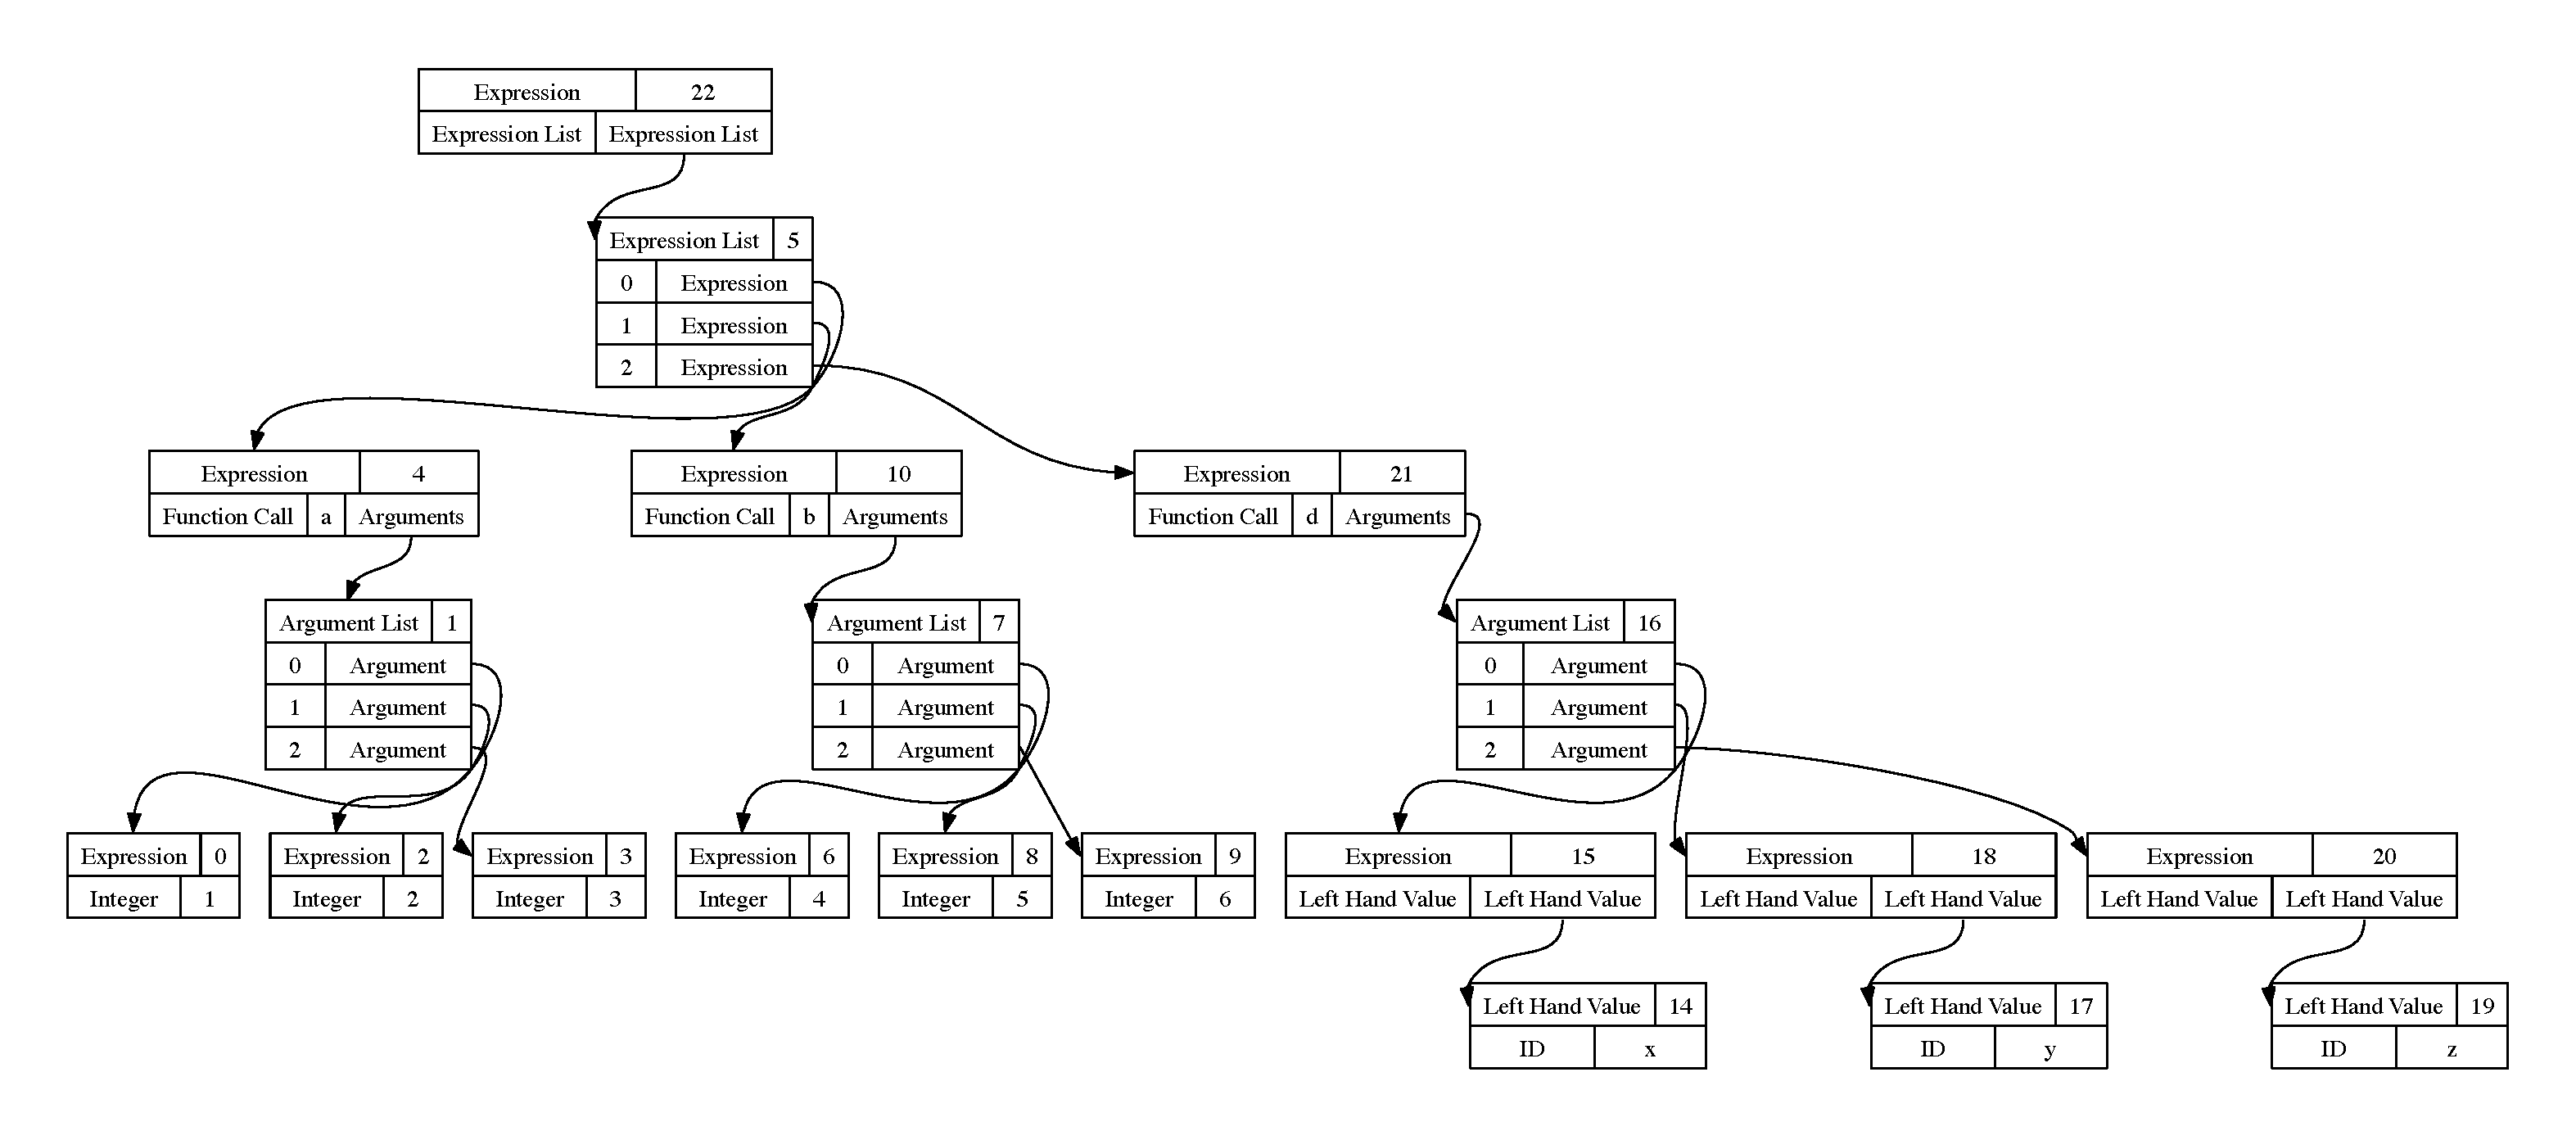
\includegraphics[width=\columnwidth]{test}  \\
对错误部分的丢弃
\end{center}

\begin{verbatim}
./graph > test.dot
====================Project Compiler T====================
=          A Tiger Language AST Graph Generator          =
=                          By                            =
=               Shengye Wang  &  Yanbo Bai               =
==========================================================
Compiler-T: Start parsing.
(a(1, 2, 3); b(4, 5, 6); c(7, 8y, 9); d(x, y, z))
Parser: syntax error, unexpected identifier, expecting "," or ")".
"y" at line 1: (a(1, 2, 3); b(4, 5, 6); c(7, 8y, 9); d(x, y, z))
               ...............................^.................
Statement discarded, continuing.
Compiler-T: Parser returned 0.
Compiler-T: 20 AST nodes created.
Compiler-T: Writing DOT script.
Compiler-T: Done. 5.000000 seconds elapsed.
==========================================================
\end{verbatim}

我们能够提示所有的词法错误(无论如何词法都会被识别成标识交给语法分析阶段,而语法阶段能够处理不合语法的错误)、语法错误。并能够修复一部分的语法错误。对于所有错误,我们均能直观地给出错位置。然而,我们尚未完成语义分析,不能判断类型上的错误。

\newpage

\section{数据结构}

数据结构及其派生关系如下,下面的这些函数是对应类的常用构造函数:

\begin{verbatim}
BasicNode(NodeType);
      Expression(ExpNodeType);
            ExpLValue(LVal*);
            ExpInteger(TInt);
            ExpNil();
            ExpString(const string&);
            ExpString(const string&);
            ExpFuncCall(const string&, ArgList*);
            ExpBinOp(Expression*, Expression*, BinOpType);
            ExpUnOp(Expression*, UnOpType);
            ExpRecord(const string&, FieldExpList);
            ExpExpList(ExpList*);
            ExpAssign(LVal*, Expression*);
            ExpIf(Expression, Expression, Expression = NULL);
            ExpWhile(Expression, Expression);
            ExpFor(const string&, Expression,
                                  Expression, Expression);
            ExpBreak();
            ExpLet(DecList*, ExpList*);
            ExpArray(const string&, Expression, Expression);
      Dec(DecNodeType _decNodeType);
            TyDec(const string&, Ty);
            VarDec(const string&, const string&, Expression*);
            VarDec(const string&, Expression*);
            FuncDec(const string&, FieldList*,
                          const string&, Expression*) ;
            FuncDec(const string&, FieldList*, Expression*);
      LVal(LValNodeType _lValNodeType);
            LValID(const string&);
            LValMember(LVal, const string&);
            LValElement(LVal, Expression*);
      Ty(TyType, string);
      Ty(TyType, FieldList*);
      ExpList();
      ArgList();
      DecList();
      FieldExpList();
      FieldList();
\end{verbatim}

上述表示中,缩进表示类的派生关系。通过设置构造函数为保护成员,只有最终的子类可以被实例化。\texttt{BasicNode}是所谓类的父节点,它带有一个全局唯一标识的ID。另外,它有一个子类型,表示它的直接派生类的类型。根据这个类型调用时可以做强制类型转换。这个类型编号必须在实例化时通过子类设置,外部可以通过公有函数读取,但不能改写。另外它拥有虚析构函数,可以通过对它的释放来释放任意一个节点。这对于错误处理时删除已经规约的规则非常有用。

表达式类,作为中间子类,继承自\texttt{BasicNode}之外,自己还有一个次级类型编号,用来标识实例的类型。通过\texttt{case}语句可以快速的确定类型,强制转换并完成相关工作。

声明类、左值类与表达式类类似,同样派生出子类。注意,\texttt{BasicNode}、表达式类、声明类、左值类均不能直接被实例化。因而程序中的实例对象一定是具体的。

所有类都有析构函数。除了释放自己所占资源外,它们还需要释放外部的资源。例如表达式列表类在析构时需要删除它管理的每一条表达式。

\section{示例}

\subsection{代码格式化器}

\subsubsection{八皇后程序格式化前}
\begin{verbatim}
/* A program to solve the 8-queens problem */

let
    var N := 8

    type intArray = array of int

    var row := intArray [ N ] of 0
    var col := intArray [ N ] of 0
    var diag1 := intArray [N+N-1] of 0
    var diag2 := intArray [N+N-1] of 0

    function printboard() =
       (for i := 0 to N-1
	 do (for j := 0 to N-1 
	      do print(if col[i]=j then " O" else " .");
	     print("\n"));
         print("\n"))

    function try(c:int) = 
( /*  for i:= 0 to c do print("."); print("\n"); flush();*/
     if c=N
     then printboard()
     else for r := 0 to N-1
	   do if row[r]=0 & diag1[r+c]=0 & diag2[r+7-c]=0
	           then (row[r]:=1; diag1[r+c]:=1; diag2[r+7-c]:=1;
		         col[c]:=r;
	                 try(c+1);
			 row[r]:=0; diag1[r+c]:=0; diag2[r+7-c]:=0)

)
 in try(0)
end
\end{verbatim}

\subsubsection{八皇后程序格式化后}
\begin{verbatim}
./formatter < testcases/queens.tig 
====================Project Compiler T====================
=               A Tiger Language Formatter               =
=                          By                            =
=               Shengye Wang  &  Yanbo Bai               =
==========================================================
Compiler-T: Start parsing.
Compiler-T: Parser returned 0.
Compiler-T: 161 AST nodes created.
Compiler-T: Rewriting Tiger source.
let
    var N := 8
    type intArray = array of int
    var row := intArray[N] of 0
    var col := intArray[N] of 0
    var diag1 := intArray[N + N - 1] of 0
    var diag2 := intArray[N + N - 1] of 0
    function printboard() = 
        (
            for i := 0 to N - 1 do
                (
                    for j := 0 to N - 1 do
                        print(if col[i] = j then
                            " O"
                        else
                            " .");
                    print("\n")
                );
            print("\n")
        )
    function try(c : int) = 
        (
            if c = N then
                printboard()
            else
                for r := 0 to N - 1 do
                    if row[r] = 0 & diag1[r + c] = 0 & diag2[r + 7 - c] = 0 then
                        (
                            row[r] := 1;
                            diag1[r + c] := 1;
                            diag2[r + 7 - c] := 1;
                            col[c] := r;
                            try(c + 1);
                            row[r] := 0;
                            diag1[r + c] := 0;
                            diag2[r + 7 - c] := 0
                        )
        )
in
    try(0)
end
Compiler-T: Done. 0.000661 seconds elapsed.
==========================================================
\end{verbatim}

\subsubsection{归并排序格式化前}
\begin{verbatim}
let 

 type any = {any : int}
 var buffer := getchar()

function readint(any: any) : int =
 let var i := 0
     function isdigit(s : string) : int = 
		  ord(buffer)>=ord("0") & ord(buffer)<=ord("9")
     function skipto() =
       while buffer=" " | buffer="\n"
         do buffer := getchar()
  in skipto();
     any.any := isdigit(buffer);
     while isdigit(buffer)
       do (i := i*10+ord(buffer)-ord("0"); buffer := getchar());
     i
 end

 type list = {first: int, rest: list}

 function readlist() : list =
    let var any := any{any=0}
        var i := readint(any)
     in if any.any
         then list{first=i,rest=readlist()}
         else nil
    end

 function merge(a: list, b: list) : list =
   if a=nil then b
   else if b=nil then a
   else if a.first < b.first 
      then list{first=a.first,rest=merge(a.rest,b)}
      else list{first=b.first,rest=merge(a,b.rest)}

 function printint(i: int) =
  let function f(i:int) = if i>0 
	     then (f(i/10); print(chr(i-i/10*10+ord("0"))))
   in if i<0 then (print("-"); f(-i))
      else if i>0 then f(i)
      else print("0")
  end

 function printlist(l: list) =
   if l=nil then print("\n")
   else (printint(l.first); print(" "); printlist(l.rest))

   var list1 := readlist()
   var list2 := (buffer:=getchar(); readlist())


  /* BODY OF MAIN PROGRAM */
 in printlist(merge(list1,list2))
end
\end{verbatim}

\subsubsection{归并排序格式化后}
\begin{verbatim}
====================Project Compiler T====================
=               A Tiger Language Formatter               =
=                          By                            =
=               Shengye Wang  &  Yanbo Bai               =
==========================================================
Compiler-T: Start parsing.
Compiler-T: Parser returned 0.
Compiler-T: 273 AST nodes created.
Compiler-T: Rewriting Tiger source.
let
    type any = {any : int}
    var buffer := getchar()
    function readint(any : any) : int = 
        let
            var i := 0
            function isdigit(s : string) : int = 
                ord(buffer) >= ord("0") & ord(buffer) <= ord("9")
            function skipto() = 
                while buffer = " " | buffer = "\n" do
                    buffer := getchar()
        in
            skipto();
            any.any := isdigit(buffer);
            while isdigit(buffer) do
                (
                    i := i * 10 + ord(buffer) - ord("0");
                    buffer := getchar()
                );
            i
        end
    type list = {first : int, rest : list}
    function readlist() : list = 
        let
            var any := any{any = 0}
            var i := readint(any)
        in
            if any.any then
                list{first = i, rest = readlist()}
            else
                nil
        end
    function merge(a : list, b : list) : list = 
        if a = nil then
            b
        else
            if b = nil then
                a
            else
                if a.first < b.first then
                    list{first = a.first, rest = merge(a.rest, b)}
                else
                    list{first = b.first, rest = merge(a, b.rest)}
    function printint(i : int) = 
        let
            function f(i : int) = 
                if i > 0 then
                    (
                        f(i / 10);
                        print(chr(i - i / 10 * 10 + ord("0")))
                    )
        in
            if i < 0 then
                (
                    print("-");
                    f(- i)
                )
            else
                if i > 0 then
                    f(i)
                else
                    print("0")
        end
    function printlist(l : list) = 
        if l = nil then
            print("\n")
        else
            (
                printint(l.first);
                print(" ");
                printlist(l.rest)
            )
    var list1 := readlist()
    var list2 := (
        buffer := getchar();
        readlist()
    )
in
    printlist(merge(list1, list2))
end
Compiler-T: Done. 0.000933 seconds elapsed.
==========================================================
\end{verbatim}

可见,对于两个测试用例,代码格式化器并没有改变代码的语义。这说明代码格式化器工作正常。由于格式化器先翻译到了抽象语法树,再从抽象语法树生成代码,因而也可以证明抽象语法树正确。

\subsection{树形图像生成器}

\begin{center}
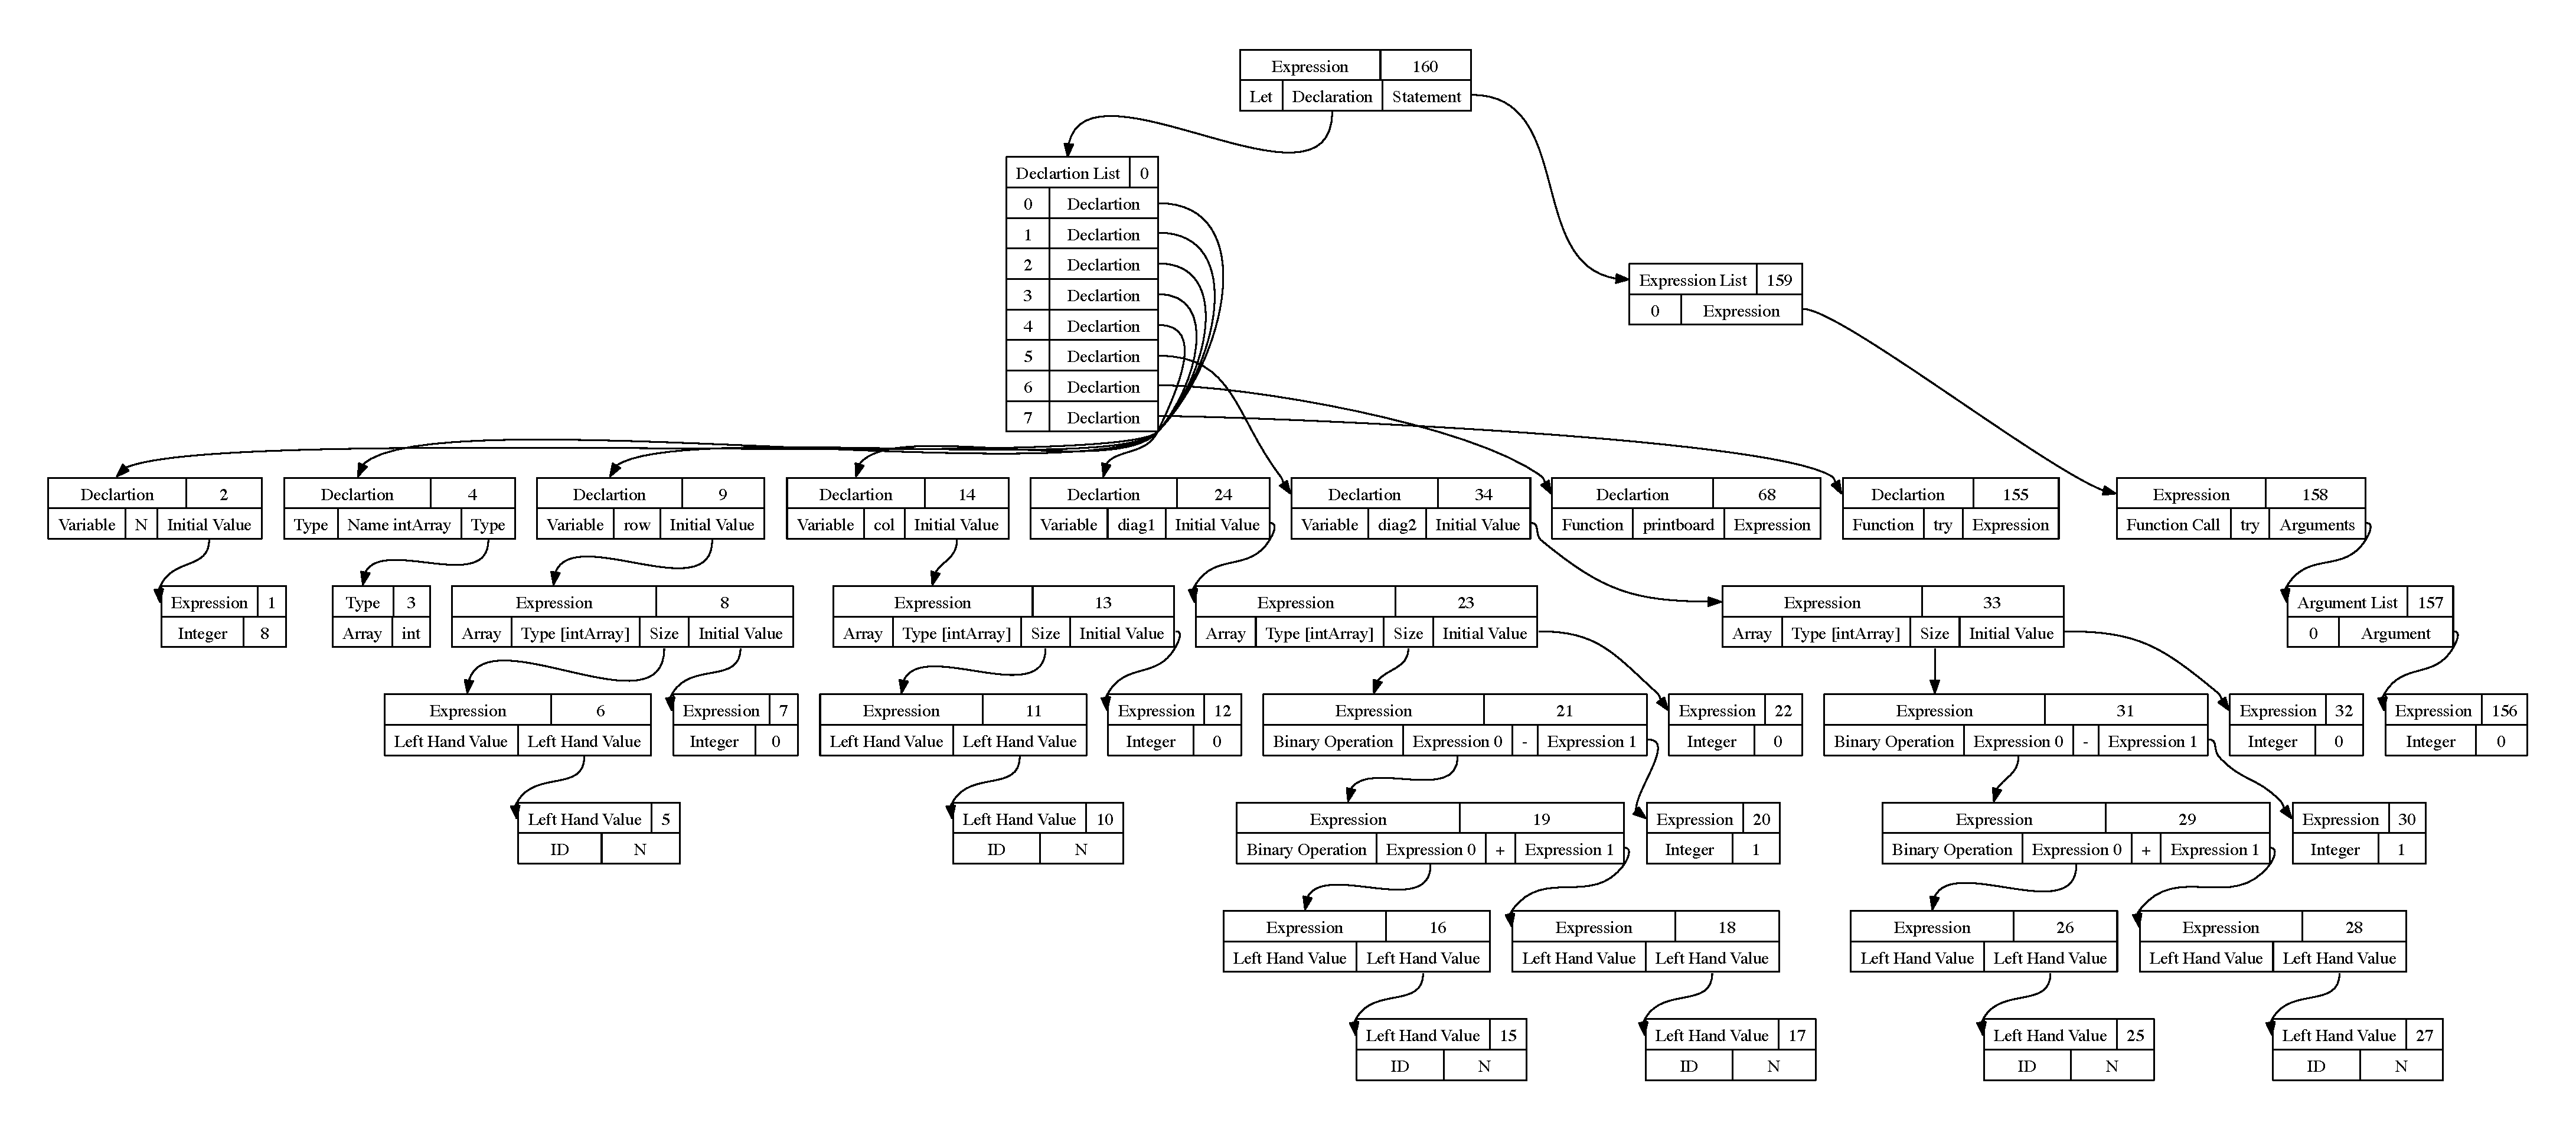
\includegraphics[width=\columnwidth]{queen}  \\
八皇后问题
\end{center}

\begin{verbatim}
./graph < queens.tig > queen.dot
====================Project Compiler T====================
=          A Tiger Language AST Graph Generator          =
=                          By                            =
=               Shengye Wang  &  Yanbo Bai               =
==========================================================
Compiler-T: Start parsing.
Compiler-T: Parser returned 0.
Compiler-T: 161 AST nodes created.
Compiler-T: Writing DOT script.
Compiler-T: Done. 0.000958 seconds elapsed.
==========================================================
\end{verbatim}

\begin{center}

\includegraphics[width=\columnwidth]{merge}  \\
归并排序
\end{center}

\begin{verbatim}
./graph < merge.tig > merge.dot
====================Project Compiler T====================
=          A Tiger Language AST Graph Generator          =
=                          By                            =
=               Shengye Wang  &  Yanbo Bai               =
==========================================================
Compiler-T: Start parsing.
Compiler-T: Parser returned 0.
Compiler-T: 273 AST nodes created.
Compiler-T: Writing DOT script.
Compiler-T: Done. 0.002452 seconds elapsed.
==========================================================
\end{verbatim}

对于每一个测试用例,生成的格式化后代码和dot代码、PDF图像均可以在Result目录下找到。

\section{心得体会}



\end{document}
